\clearpage
\section{Hardware Plattform}\label{sec:HardwarePlattform}
\todo[inline]{Cyrill}

\todo[inline]{Übersicht über die eingesetzte Hardware. Einleitung inkl. Erläuterung Unterschiede und Gemeinsamkeiten P2P und Mesh Test Hardware (Stichwort: Open Source, Open Hardware).}

Für den Benchmark und den Vergleich der drei Mesh Protokolle sowie die P2P Testinfrastruktur wird eine einheitliche Hardwareplattform verwendet. Dies macht ein Vergleich der Testresultate möglich. Im Zentrum steht dabei der nRF52840 SoC von Nordic Semiconductor welcher eine voll umfängliche Plattform für Bluetooth und IEEE 802.15.4 darstellt. Damit besonders die P2P Testinfrastruktur einfach nutzbar ist, werden Entwicklungsboards vom Chip Hersteller eingesetzt welche vergleichsweise günstig und gut verfügbar sind. Nachfolgend wird auf die Hardware und deren Einsatz genauer eingegangen.


\subsection{System on Chip}\label{subsec:SystemonChip}

Der nRF52840 ist ein Highend System-on-Chip welcher gleichermassen Bluetooth 5 wie auch den IEEE 802.15.4 Wireless-Personal-Area-Network (WPAN) Standard unterstützt. Auf Wunsch sogar als Multiprotocol Lösung.
Entscheidend für die vorliegende Anwendung ist, dass der SoC von den drei Organisationen Bluetooth SIG, Openthread und der Zigbee Alliance offiziell für das jeweilige Protokoll zertifiziert ist.
Die Eckdaten des nRF52840 SoC sind in der Tabelle \ref{tab:EigenschaftennRF52840SoC} kurz zusammengefasst.

\begin{table}[h]
\centering
\begin{tabular}{ll}
\toprule
Microcontroller    & 32-bit ARM Cortex-M4F                        \\
Clock frequency    & 64 MHz                                       \\
Flash              & 1MB                                        \\
RAM                & 256kB                                          \\
Frequency Band     & 2.4GHz                                       \\
Wireless protocols & IEEE 802.15.4 (Thread, Zigbee), Bluetooth 5.0  \\
\bottomrule
\end{tabular}
\caption{Eigenschaften nRF52840 SoC \cite{nordic_semiconductor_asa_nrf52840_2020}}
\label{tab:EigenschaftennRF52840SoC}
\end{table}


\subsection{Hardware Development Kits}\label{subsec:HardwareDevelopmentKits}

Der Hersteller Nordic Semiconductor bietet gleich zwei Entwicklungsboards für den SoC an. Einerseits das umfangreiche nRF52840-DK (pca10056) \ref{fig:nrf52840-DK} welches zusammen mit dem Software Development Kit von Nordic Semiconductor eine vollumfängliche Entwicklungsumgebung bietet.
Auf dem Board ist nebst diverser Peripherie auch ein Segger J-Link Debugger integriert.
Dieser erleichtert das flashen und debuggen ungemein.
Im Benchmark Betrieb fungiert ein nRF52840-DK als Benchmark Master Node \ref{subsubsec:Nodes} wobei die USB-UART Schnittstelle als Interface zur Benchmark Management Station verwendet wird.
Als einfachere Alternative zum voll umfänglichen Development Kit werden als Benchmark Slave Nodes \ref{subsubsec:Nodes} die einfacheren und günstigeren nRF52840-Dongle (pca10059) \ref{fig:nrf52840-Dongle} verwendet.
Offensichtlich als USB-Dongle entworfen können die Dongles flexibel eingesetzt werden. Die fehlende Peripherie macht die Hardware jedoch unpassend für die Entwicklung neuer Firmware.
Beide Typen von Entwicklungsboards besitzen eine integrierte PCB Antenne wenn auch in unterschiedlichen Ausführungen.
Im Abschnitt \ref{subsec:AntenneundStrahlungscharakteristik} wird näher auf die Ausführung der Antennen und deren Strahlungscharakteristik eingegangen.


\begin{figure}[!htbp]
\centering
\begin{minipage}[b]{0.49\textwidth}
		\centering
		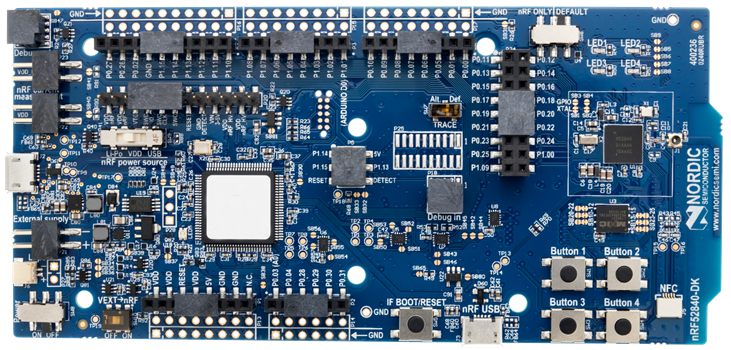
\includegraphics[width=\textwidth]{nRF52840_DK.png}
		\caption[nRF52840-DK PCA10056]{PCA10056 \cite{nordic_semiconductor_asa_nrf52840_2020-1}}
		\label{fig:nrf52840-DK}
\end{minipage}
\begin{minipage}[b]{0.49\textwidth}
		\centering
		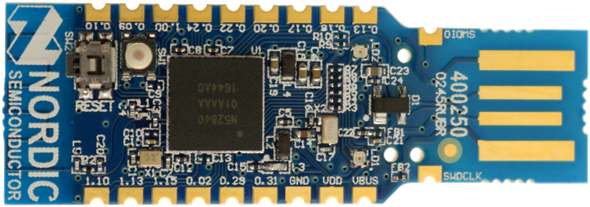
\includegraphics[width=0.9\textwidth]{nRF52840_Dongle_gerade.png}
		\caption[nRF52840-Dongle PCA10059]{PCA10059 \cite{nordic_semiconductor_asa_nrf52840_2020-2}}
		\label{fig:nrf52840-Dongle}
\end{minipage}
\end{figure}



\subsection{Aufbau Testnode}\label{subsec:AufbauTestnode}

Der Aufbau des Testnodes wie er in Abbildung \ref{fig:TestnodenRF52840-DongleinklBatteriepack} wurde so einfach wie möglich gehalten. Ein externes Batteriepaket wird eingesetzt, damit der Benchmark Slave Node unabhängig von einer externen Stromversorgung betrieben werden kann. So kann der Einsatzort frei gewählt und auch kurzfristig geändert werden.
Das Batteriepaket besteht aus zwei Standard Mignon Einwegzellen vom Typ AA mit je 1.5V Spannung. In Serieschaltung betrieben wird die Speisespannung von 3V erreicht welche für den Dongle ausreichend ist. Mit fortschreitender Entladung der Zellen sinkt die Spannung. Da der SoC einen Betriebsspannungsbereich von 1.7V bis 5.5V hat stellt die sinkende Spannung jedoch kein Problem dar.
Die Speisung des nRF52840-Dongle erfolgt über einen 2-poligen JST Header der gemäss Datenblatt xx mit dem VDD OUT und GND Anschluss verbunden ist. Am VDD OUT Anschluss ist ein Betriebsspannungsbereich von 1.8V bis 3.6V zulässig.
Das Batteriegehäuse verfügt ausserdem über einen Schalter um den Testnode nach Belieben ein- und auszuschalten.
Mit den verwendeten Batterien welche je eine Kapazität von 2900mAh besitzen, können die Nodes im Mesh Benchmark Betrieb über mehrere Tage betrieben werden \cite{distrelec_schweiz_ag_rnd_2020}.
Eine Messung des Stromverbrauches im Benchmark Betrieb hat gezeigt, dass dieser bei 3V Batteriespannung durchschnittlich 15mA beträgt. Dieser relativ hohe Wert wird einerseits verursacht durch die LED's die geschaltet werden und andererseits durch das Radio Interface welches im Leerlauf permanent im Empfangsmodus ist um allfällige Start Messages empfangen zu können. 
Dieser Verbrauch ermöglicht eine Betriebsdauer von rund 190 Stunden was mehr als ausreichend ist für diese Verwendung.

\begin{figure} [H]
	\centering
	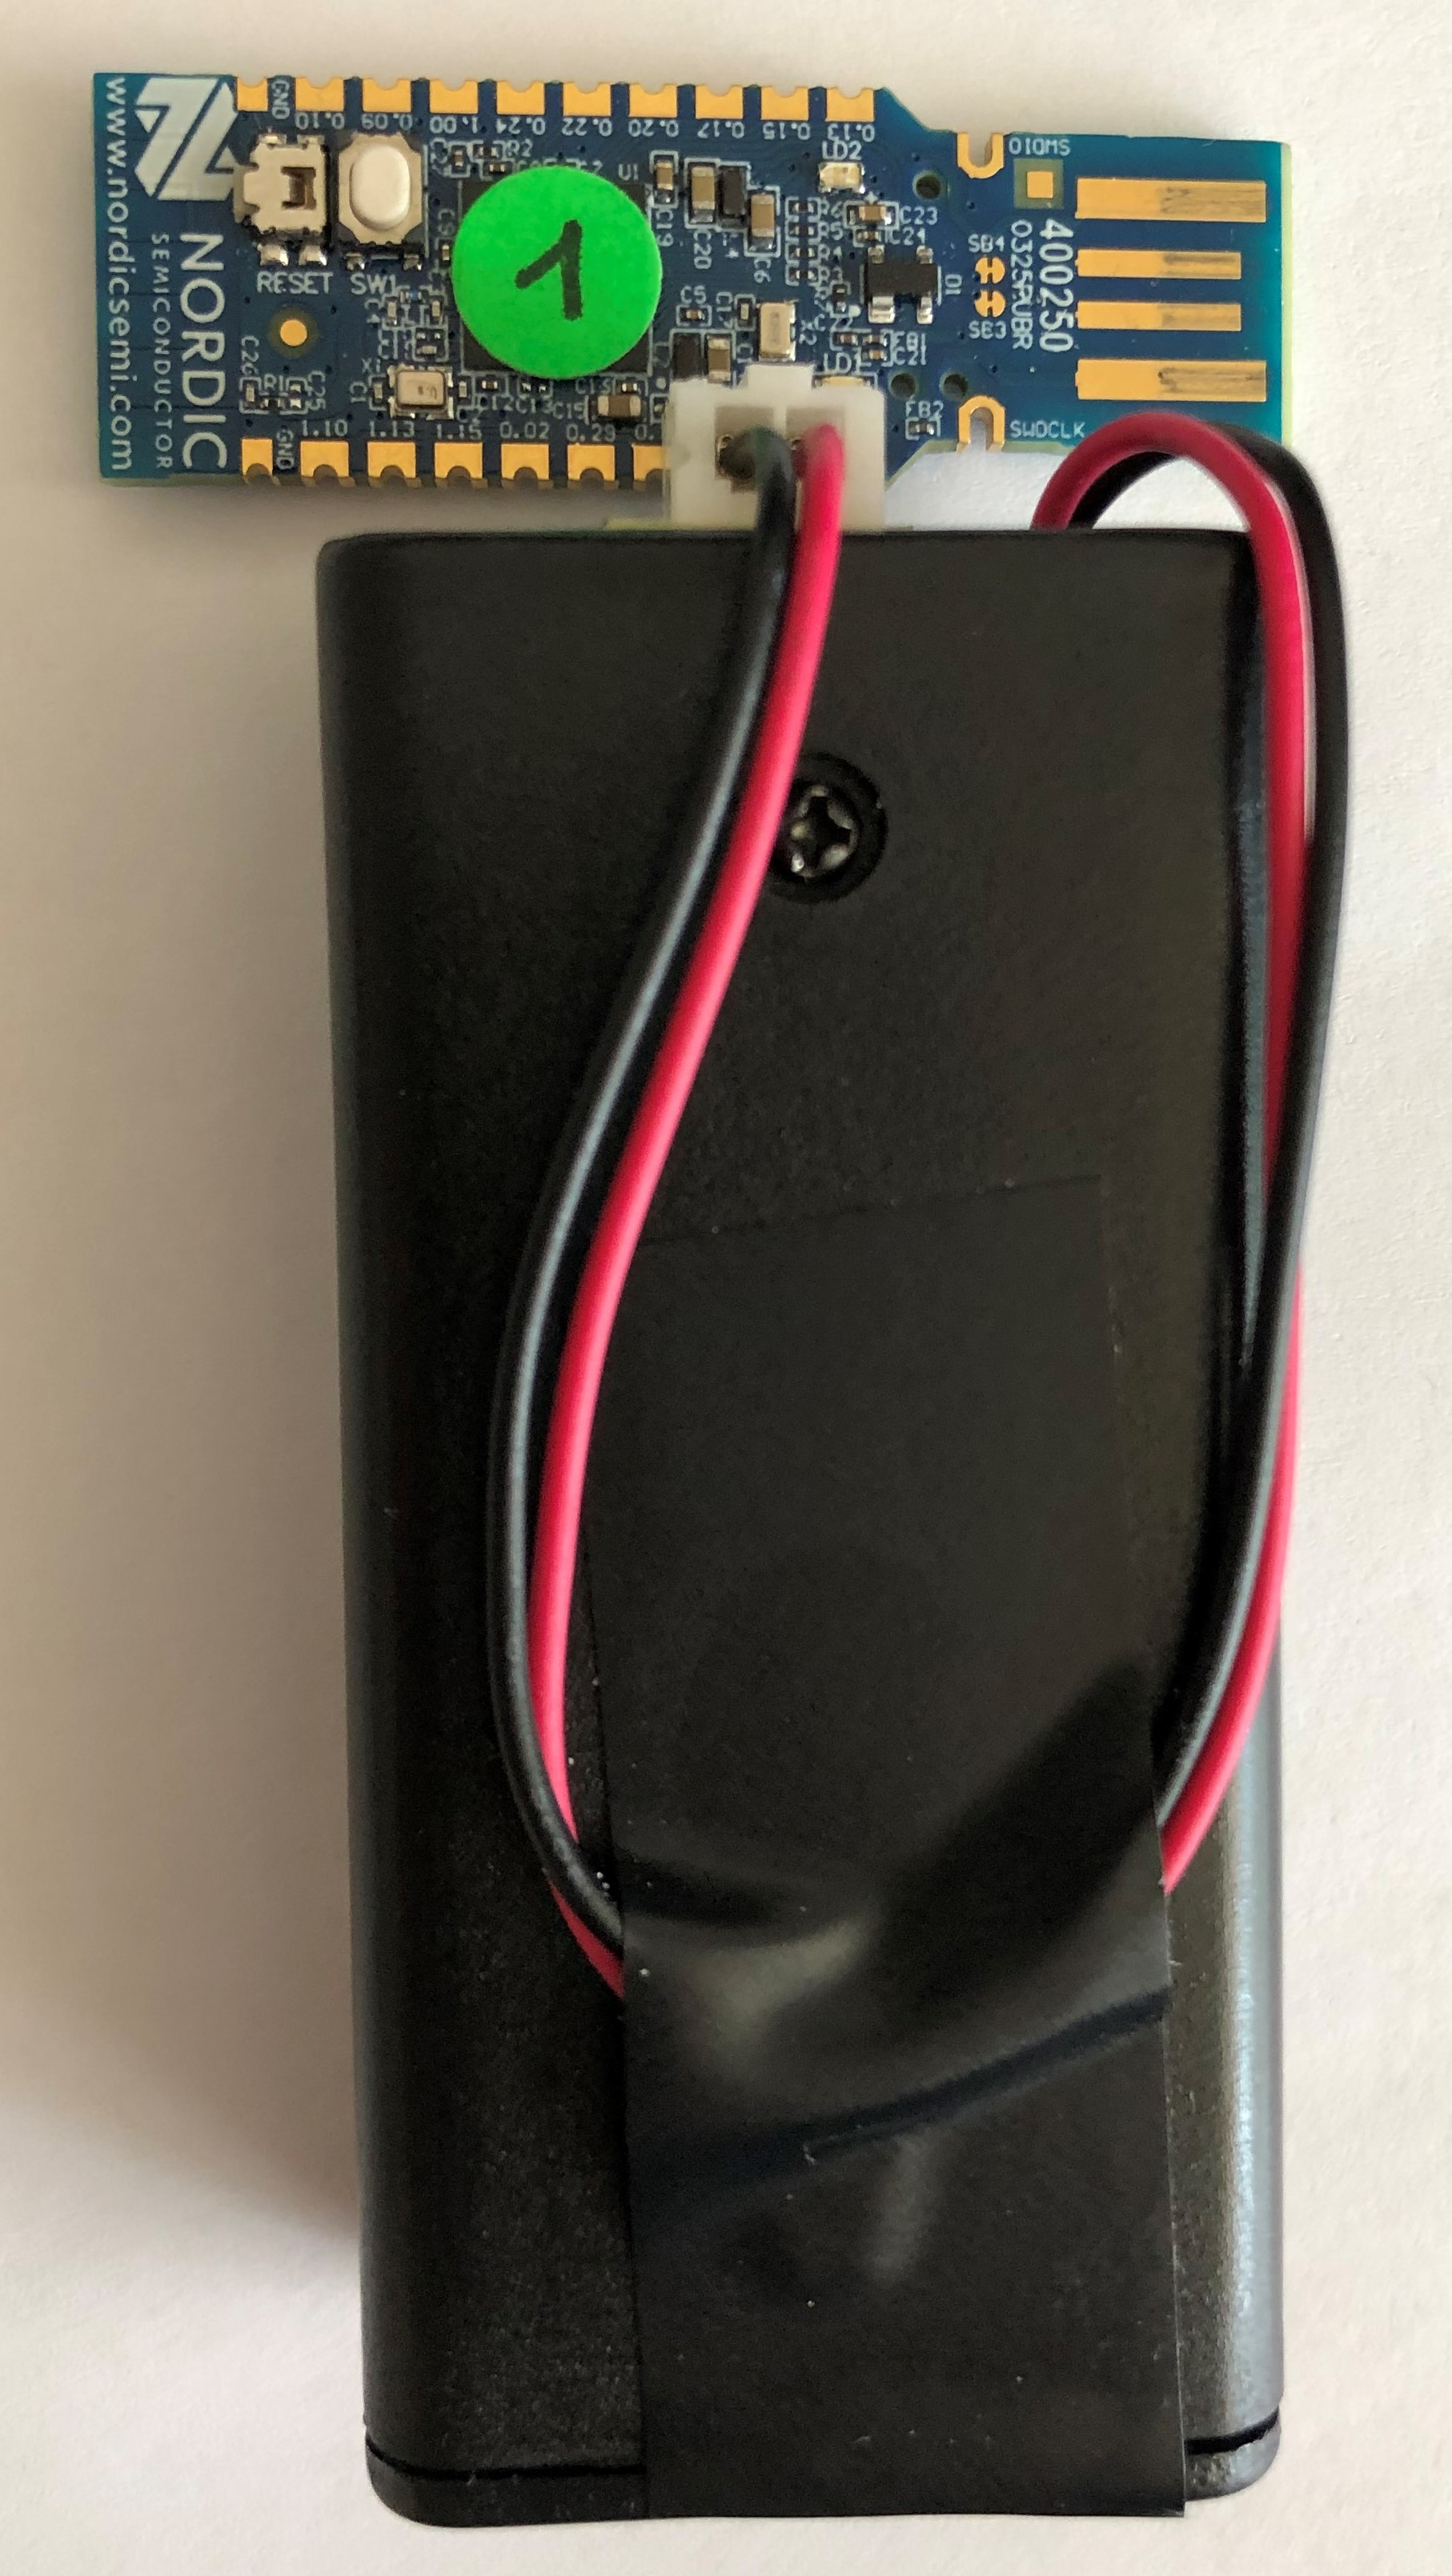
\includegraphics[width=0.2\textwidth]{Node_picture.png}
	\caption{Testnode: nRF52840-Dongle inkl. Batteriepack}
	\label{fig:TestnodenRF52840-DongleinklBatteriepack}
\end{figure}

Die Befestigung des Dongles am Batteriepaket erfolgte so dass die PCB Antenne welche sich am Ende des PCB's befindet möglichst frei liegt und sich dadurch die bestmöglichen Abstrahlungseigenschaften ergeben. Ein weiterer Vorteil der in Abbildung \ref{fig:TestnodenRF52840-DongleinklBatteriepack} dargestellten Montage ist die Zugänglichkeit des USB Ports. So können die Benchmark Nodes auf einfachste Arte und Weise mit einer neuen Software geflasht werden.

 
\subsection{Antenne und Strahlungscharakteristik}\label{subsec:AntenneundStrahlungscharakteristik}

Wie bereits im Abschnitt \ref{subsec:HardwareDevelopmentKits} erwähnt, besitzen die beiden eingesetzten Development Kits jeweils eine PCB Antenne. Beim nRF52840-DK ist diese als einfache IFA (Inverted-F Antenna) \ref{fig:nrf52840-DK-Copper} ausgeführt während dem der Dongle mangels Platz auf dem PCB eine sogenannte MIFA (Meandered Inverted-F Antenna) \ref{fig:nrf52840-Dongle-Copper} besitzt.

\begin{figure}[!htbp]
\centering
\begin{minipage}[b]{0.49\textwidth}
		\centering
		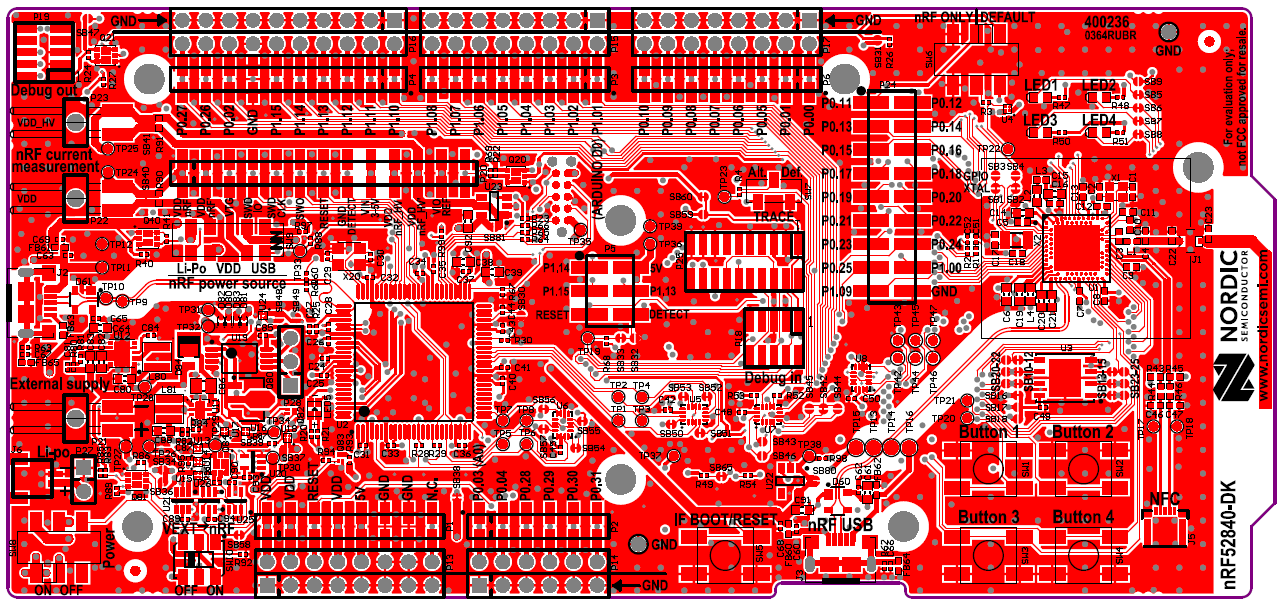
\includegraphics[width=\textwidth]{nRF52840_DK_Copper.png}
		\caption[PCA10056 Copperplane mit IFA-Antenne]{PCA10056 Copperplane \cite{nordic_semiconductor_asa_pca10056_schematic_and_pcb_2019}}
		\label{fig:nrf52840-DK-Copper}
\end{minipage}
\begin{minipage}[b]{0.49\textwidth}
		\centering
		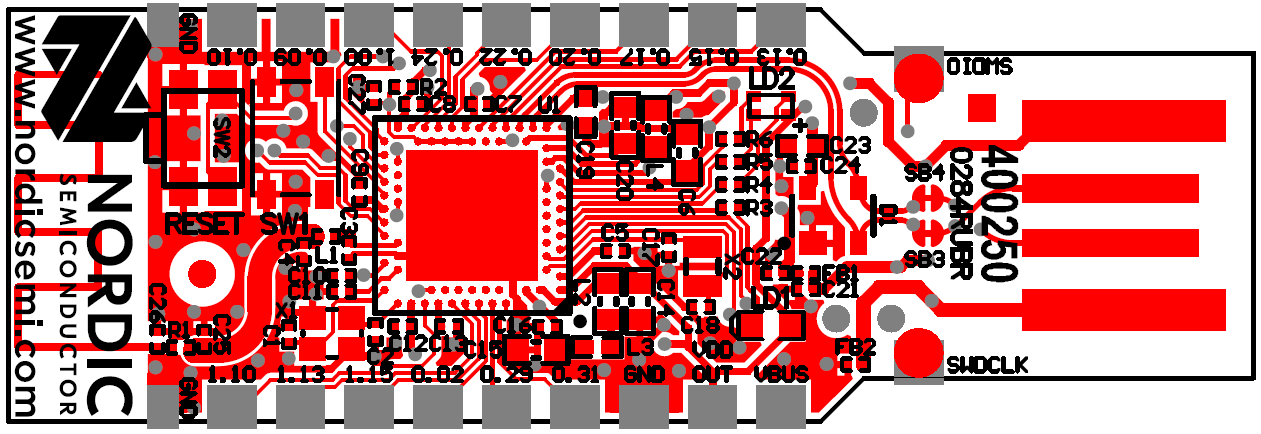
\includegraphics[width=0.9\textwidth]{nRF52840_Dongle_Copper.png}
		\caption[PCA10059 Copperplane mit MIFA-Antenne]{PCA10059 Copperplane \cite{nordic_semiconductor_asa_pca10059_schematic_and_pcb_2020}}
		\label{fig:nrf52840-Dongle-Copper}
\end{minipage}
\end{figure}

Erste Versuche zu Beginn dieser Projektarbeit haben gezeigt, dass sich die Eigenschaften der beiden Antennen relativ deutlich unterscheiden. Beispielweise konnte festgestellt werden, dass die Antenne des pca10056 eine deutlich höhere Reichweite erzielt als jene des pca10059.
Um diese Vermutungen zu prüfen wurde eine Spektrumanalyse der gestrahlten Emmission an den beiden Entwicklungsboards durchgeführt. Diese Messungen wurden im Rahmen eines Projektes für das Modul emv durchgeführt und dort in einem Bericht dokumentiert. Nachfolgend werden die wichtigsten Erkenntnisse daraus nochmals wieder gegeben. Der ganze Bericht ist im Anhang \ref{app:BerichtemvMessungDevelopmentKits} zu finden.

Bei den durchgeführten Messungen lag das Hauptaugenmerk auf der Erfassung der Abstrahlcharakteristik in dreidimensionaler Richtung. Die absoluten Signalpegel konnten dabei nicht korrekt erfasst werden, waren jedoch auch nicht von grosser Bedeutung.
Die in den beiden Abbildungen \ref{fig:PCA10056Peak} und \ref{fig:PCA10059Peak} dargestellten Abstrahlcharakteristiken der jeweiligen Development Boards zeigen deutliche Unterschiede auf. Während das pca10056 eine sehr gleichmässige Verteilung der Sendeleistung über die gesamte Halbkugeloberfläche ausweist, zeigt das pca10059 deutliche Schwachstellen in Form von Dellen in der Halbkugel auf.
Weiter unterscheidet sich der maximal Wert in Z-Richtung zwar optisch nur minimal, in Wirklichkeit bedeutet dies jedoch eine 2 bis 4 fach höhere Dämpfung und somit eine deutlich kleinere Reichweite.



\begin{figure}[!htbp]
\centering
\begin{minipage}[b]{0.49\linewidth}
	\centering
	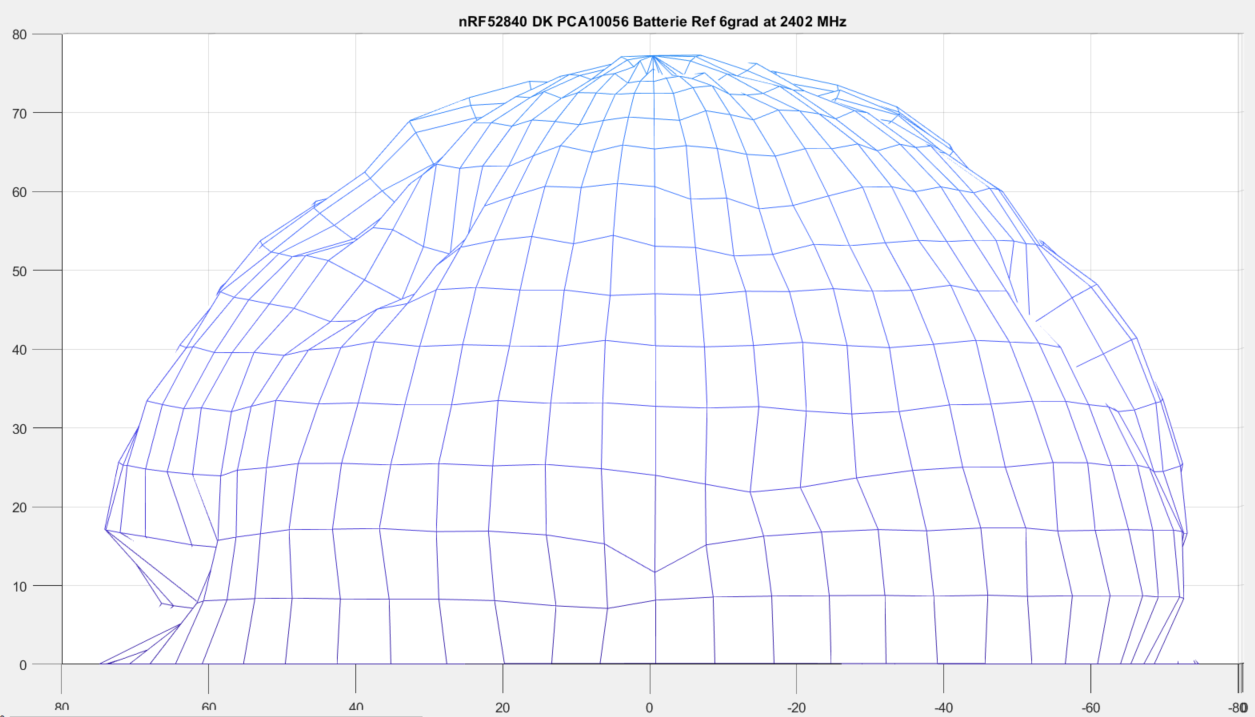
\includegraphics[width=\textwidth]{PCA10056_Peak.png}
	\caption{Abstrahlung in Z-Richtung PCA10056}
	\label{fig:PCA10056Peak}
\end{minipage}
\begin{minipage}[b]{0.49\linewidth}
	\centering
	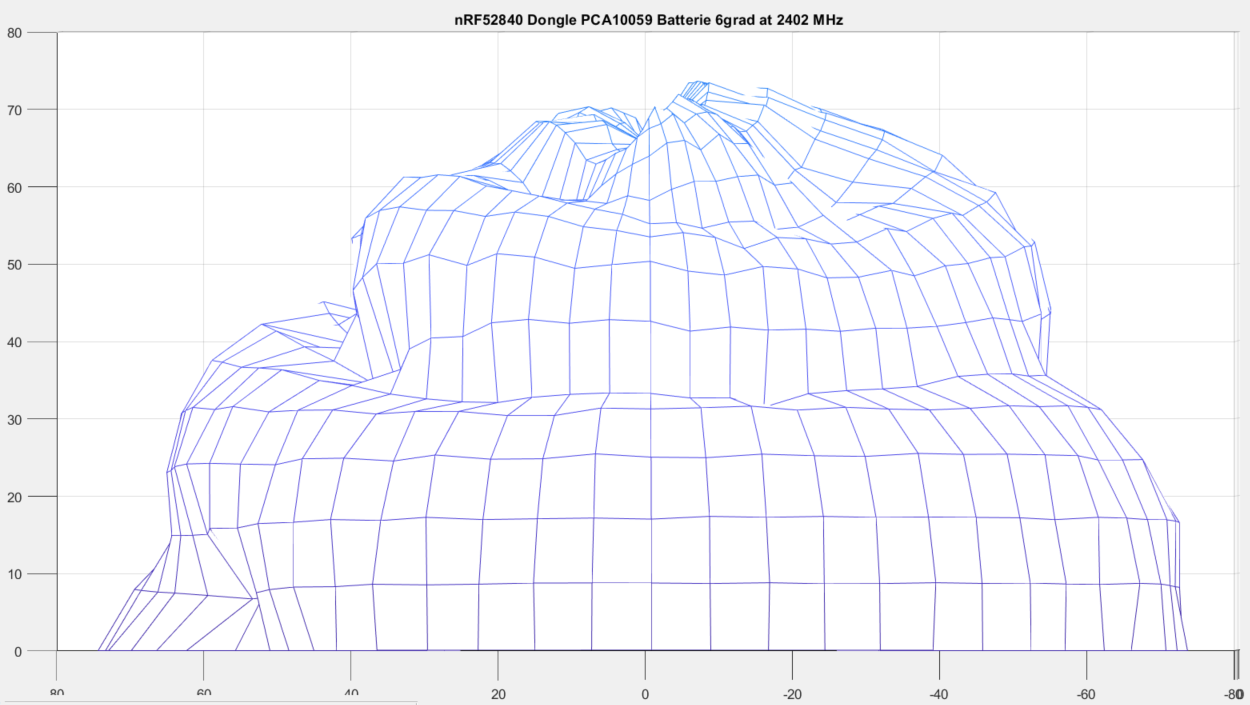
\includegraphics[width=\textwidth]{PCA10059_Peak.png}
	\caption{Abstrahlung in Z-Richtung PCA10059}
	\label{fig:PCA10059Peak}
\end{minipage}
\end{figure}

Die gemessenen Abstrahleigenschaften der beiden Antennen bestätigen schliesslich unsere Erfahrungen die wir mit den Boards bereits gemacht haben. Die MIFA Antenne des pca10059 weisst einige klare Nachteile gegenüber der IFA Antenne des pca10056 auf. Bei eingeschränkten Platzverhältnissen wie sie auf dem pca10059 und bei vielen Low-Power Mesh Anwendungen herrschen, ist jedoch eine MIFA eine solide Alternative.

Die Erkenntnisse aus den vorliegenden Messungen waren hilfreich bei der Planung und Durchführung der Mesh Benchmarks. Beim Aufbau der Testnodes \ref{subsec:AufbauTestnode} flossen diese beispielsweise ein um die Ausrichtung der Antenne zu optimieren. Weiter halfen die Ergebnisse bei der Interpretation der weiteren Messungen da auch dort klar aufgezeigt werden konnte, dass die Positionierung und Ausrichtung der Antenne von entscheidender Bedeutung für die Performance ist.

\subsection{Benchmark Management Station}\label{subsec:BenchmarkManagementStation}

Die Benchmark Management Station (BMS) ist im Mesh Benchmark und in der P2P Testinfrastruktur unterschiedlich ausgeführt. Im Mesh Benchmark handelt es sich um einen PC welcher via USB UART Verbindung mit dem Benchmark Master Node (BMN) verbunden ist. Dazu kann jeder PC verwendet werden.
Bei der P2P Testinfrastruktur stellt die BMS ein Raspberry Pi4 dar. Dieser wird ebenfalls wia USB UART mit dem BMN verbunden. Mit dem Einsatz eines Raspberry Pi's als BMS wird diese unabhängiger und kann einfach portiert werden. So kann die Testinfrastruktur als Messinstrument eingesetzt werden.

